\documentclass{beamer}

\mode<presentation>
{
	\usetheme{Warsaw}
	\setbeamercovered{Ilmenau}
}

\usepackage[english]{babel}
\usepackage[latin1]{inputenc}
\usepackage{times}
\usepackage[T1]{fontenc}
\usepackage{url}

% short title - long title
\title[Swift Fox]{Swift Fox}
% subtitle
\subtitle{Programming sensor networks for fun and profit}
% authors
\author[\url{http://nslvm2.cs.columbia.edu}]
{
	Marcin Szczodrak\inst{1}	\and
	Vasileios P. Kemerlis\inst{1}	\and \\
	Xuan Linh Vu\inst{2}		\and
	Yiwei Gu\inst{2}
}
% affiliations
\institute[Columbia University]
{
	Programing Languages and Translators (PLT)	\\
	Computer Science Department			\\
 	Columbia University				\and
	\inst{1}
	\{\textit{msz}, \textit{vpk}\}\texttt{@cs.columbia.edu}		\\
	\inst{2}
	\{\textit{xv2103}, \textit{yg2181}\}\texttt{@cs.columbia.edu}
}
% date
\date[PLT 2010]{04/26/2010}
% subject text in PDF info
\subject{Swift Fox presentation}
% logo
\pgfdeclareimage[height=1cm]{sf-logo}{fig/sf_logo}
\logo{\pgfuseimage{sf-logo}}
% table of contents at the beginning of each section
\AtBeginSection[]
{
	\begin{frame}<beamer>{Outline}
		\tableofcontents[currentsection,currentsubsection]
	\end{frame}
}
% uncover everything in a step-wise fashion
%\beamerdefaultoverlayspecification{<+->}


\begin{document}


\begin{frame}
	\titlepage
\end{frame}

\begin{frame}{Outline}
	\tableofcontents
	% useful option [pausesections]
\end{frame}


\section[Introduction]{Introduction (Marcin Szczodrak)}

\subsection[Overview]{Overview}

\begin{frame}{Wireless Sensor Networks}{What are they?}
	\begin{itemize}
	\item wireless ad-hoc networks
	\begin{block}{multipurpose sensor nodes (\textit{motes})}
		\begin{itemize}
		\item small
		\item low-cost, low-power
		\item self-organizing capabilities
		\end{itemize}
	\end{block}
	\item ultimately at the size of a grain of sand
	(\textit{smart dust})
	\begin{figure}
		\begin{center}
		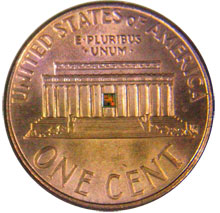
\includegraphics[scale=0.2]{fig/mote.jpg}
		\end{center}
		\caption{Tiny mote (courtesy of MIT Technology Review)}
	\end{figure} 
	\end{itemize}
\end{frame}

\subsection[Problem statement]{Problem statement}

\begin{frame}{Wireless Sensor Networks}{Why bother?}
	\begin{itemize}
	\item WSNs are pervasive
		\begin{itemize}
		\item military (battlefield surveillance, reconnaissance)
		\item environment (pollution monitoring, chemical
			detection)
		\item home automation (``smart home'')
		\item commercial domain 
		\end{itemize}
	\end{itemize}
	\begin{block}{but...}
		\begin{itemize}
		\item no standardized system facilities
		\item absence of high-level abstractions
		\item ``single'' image implementations
		\end{itemize}
	\end{block}
\end{frame}

\subsection[Swift Fox]{Swift Fox language}

\begin{frame}{Swift Fox}{Bringing back the fun in WSN programming}
	\begin{itemize}
	\item simple, event-driven language for describing
		reconfiguration policies for WSNs
	\begin{figure}
		\begin{center}
		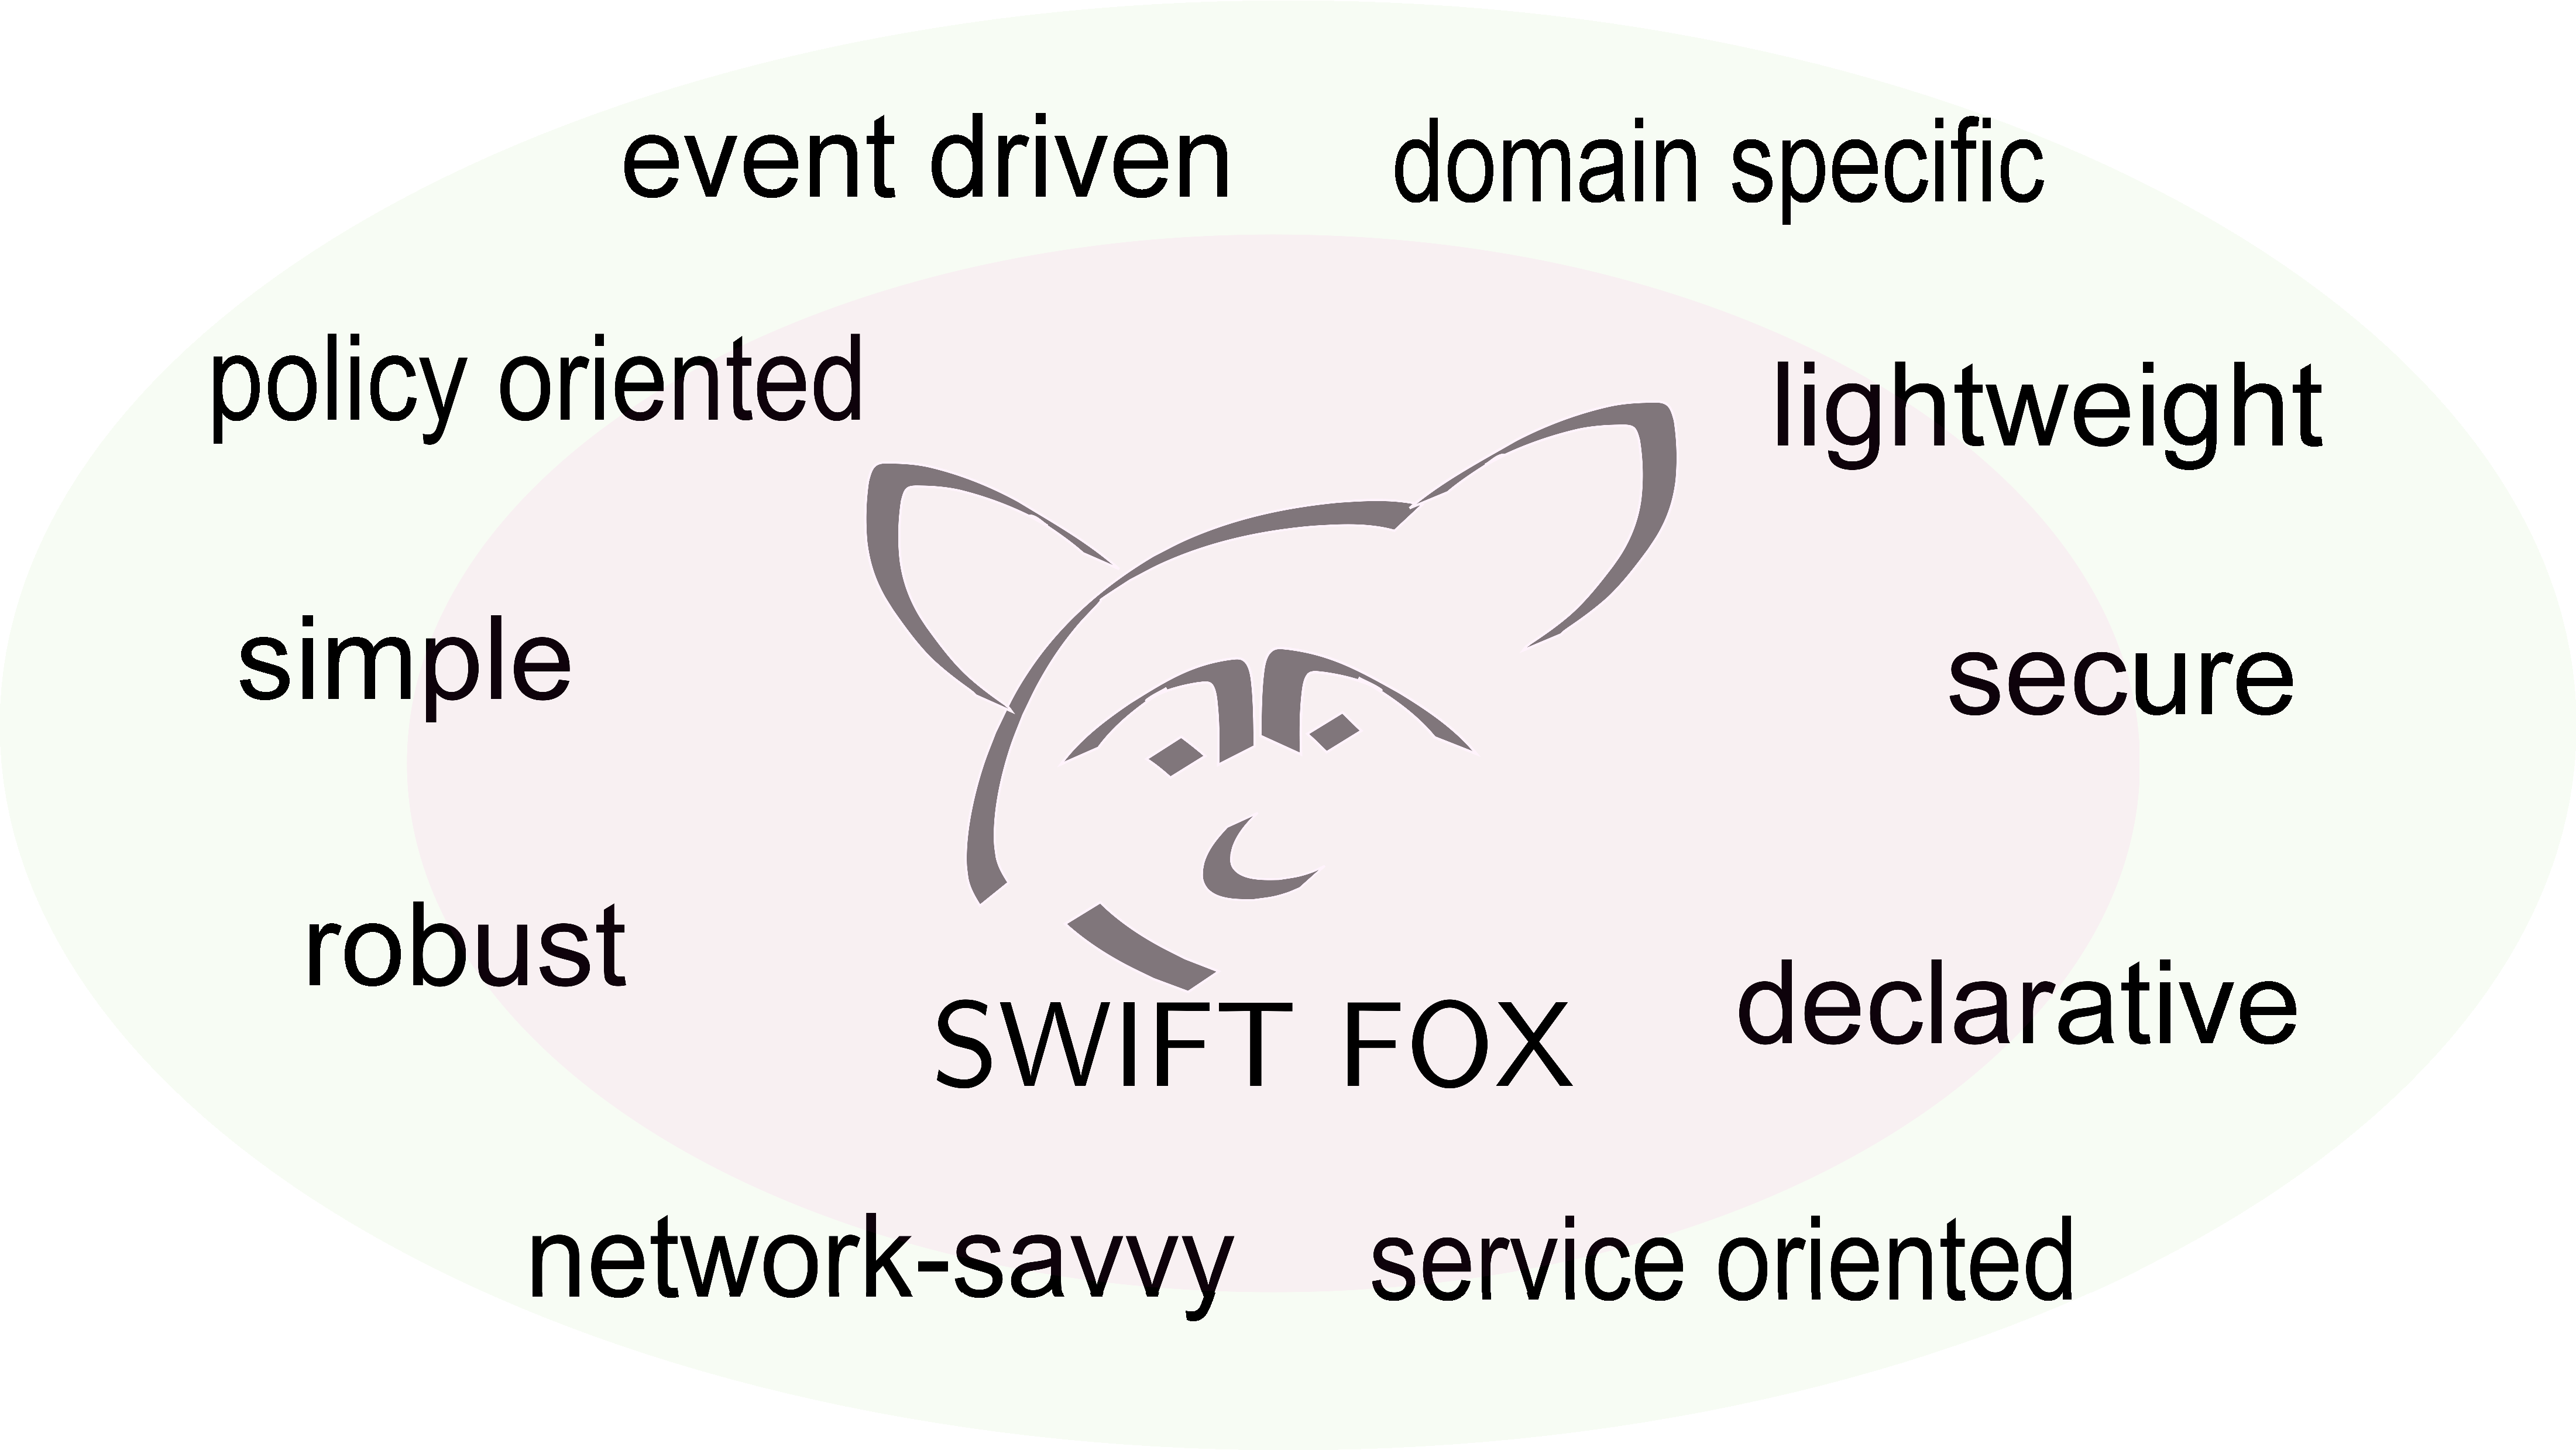
\includegraphics[scale=0.1]{fig/buzz.pdf}
		\end{center}
		\caption{Buzzwords for Swift Fox}
	\end{figure} 

	\end{itemize}
\end{frame}

\begin{frame}{Swift Fox}{Distinctive characteristics}
	\begin{itemize}
	\item simple, simple, simple
	\item enables code/logic re-use
	\item releases the programmer from the burden of dealing with WSN
	OS internals, event handling, data scatter/gather, network and
	routing protocol details
	\end{itemize}
	\begin{block}{\textbf{first} programming language for WSN
	applications}
		\begin{itemize}
		\item solve the ``problem'' and avoid plumbing
		\end{itemize}
	\end{block}
\end{frame}


\section[Language internals]{Language internals (Vasileios Kemerlis)}

\subsection[Constructs]{Language constructs}

\begin{frame}{Swift Fox}{Essential constructs}
	\begin{itemize}
	\item \textbf{configuration}: \textit{binding} between an
	application and a network protocol
	\item \textbf{event-condition}: \textit{predicate} that becomes
	true when a specific sensor reading satisfies a condition
	\item \textbf{policy}: \textit{transition} specification between
	different configuration, upon event-conditions
	\end{itemize}
	\begin{example}
		\begin{itemize}
		\item \textbf{configuration} \textit{too-cold}
		\{Send-Temp CTP\}
		\item \textbf{event-condition} \textit{cold-day}
		\{Temperature < 70F\}
		\item \textbf{from} \textbf{any} \textbf{goto}
		\textit{too-cold} \textbf{when} \textit{cold-day}
		\end{itemize}
	\end{example}
\end{frame}

\subsection[Syntax]{Syntactic structures}

\begin{frame}[fragile]
\tiny
	\begin{figure}
	\begin{center}
\begin{verbatim}
# define configurations
configuration sleep-day {nothing CTP}
configuration sleep-night {nothing CTP}
configuration too-cold {Send-Temp CTP}

# define time passing events
event-condition day {Timer = 16hr}
event-condition night {Timer = 8hr}

# define temperature sensing events
event-condition cold-day {Temperature < 70F }
event-condition cold-night {Temperature < 60F }

# reconfiguration policies
from any goto sleep-day when day
from any goto sleep-night when night
from sleep-day goto too-cold when cold-day
from sleep-night goto too-cold when cold-night
from too-cold goto sleep-day when not cold-day
from too-cold goto sleep-night when not cold-night

# and finally, the initial configuration
start sleep-day
\end{verbatim}
	\end{center}
	\end{figure}
\end{frame}

\begin{frame}{Swift Fox}{Example tree}
	\begin{figure}
		\begin{center}
		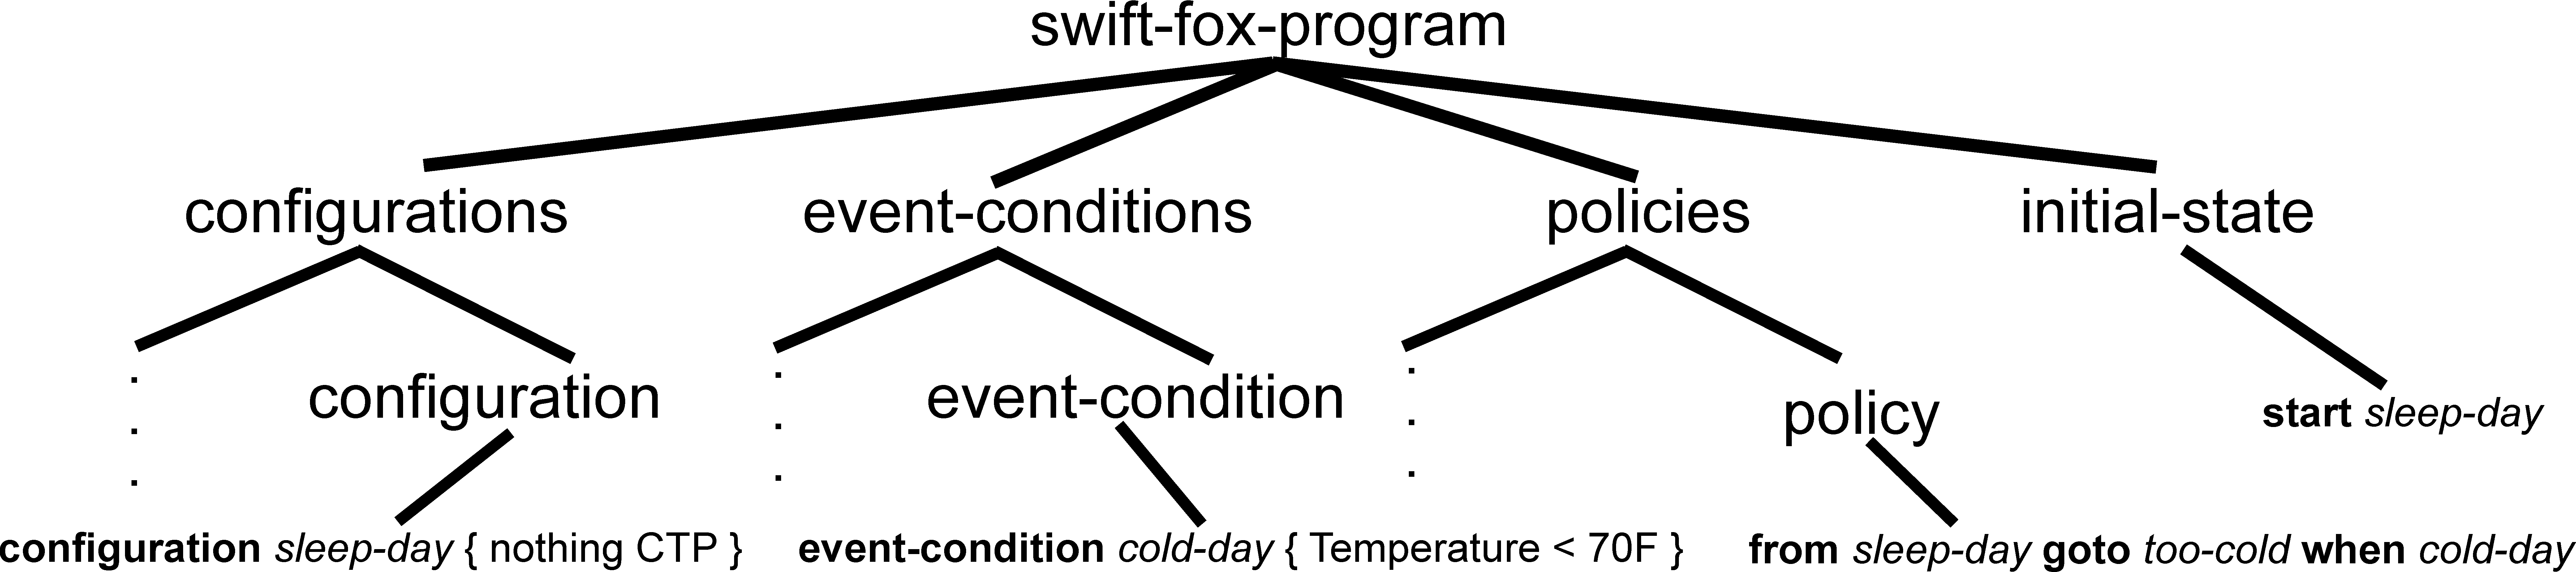
\includegraphics[scale=0.08]{fig/tree.pdf}
		\end{center}
		\caption{AST for the previous code snippet}
	\end{figure} 
\end{frame}


\section[Compiler details]{Compiler details (Yiwei Gu)}

\subsection[Compiler architecture]{Compiler architecture}

\begin{frame}{Swift Fox}{Compiler block diagram}
	\begin{figure}
		\begin{center}
		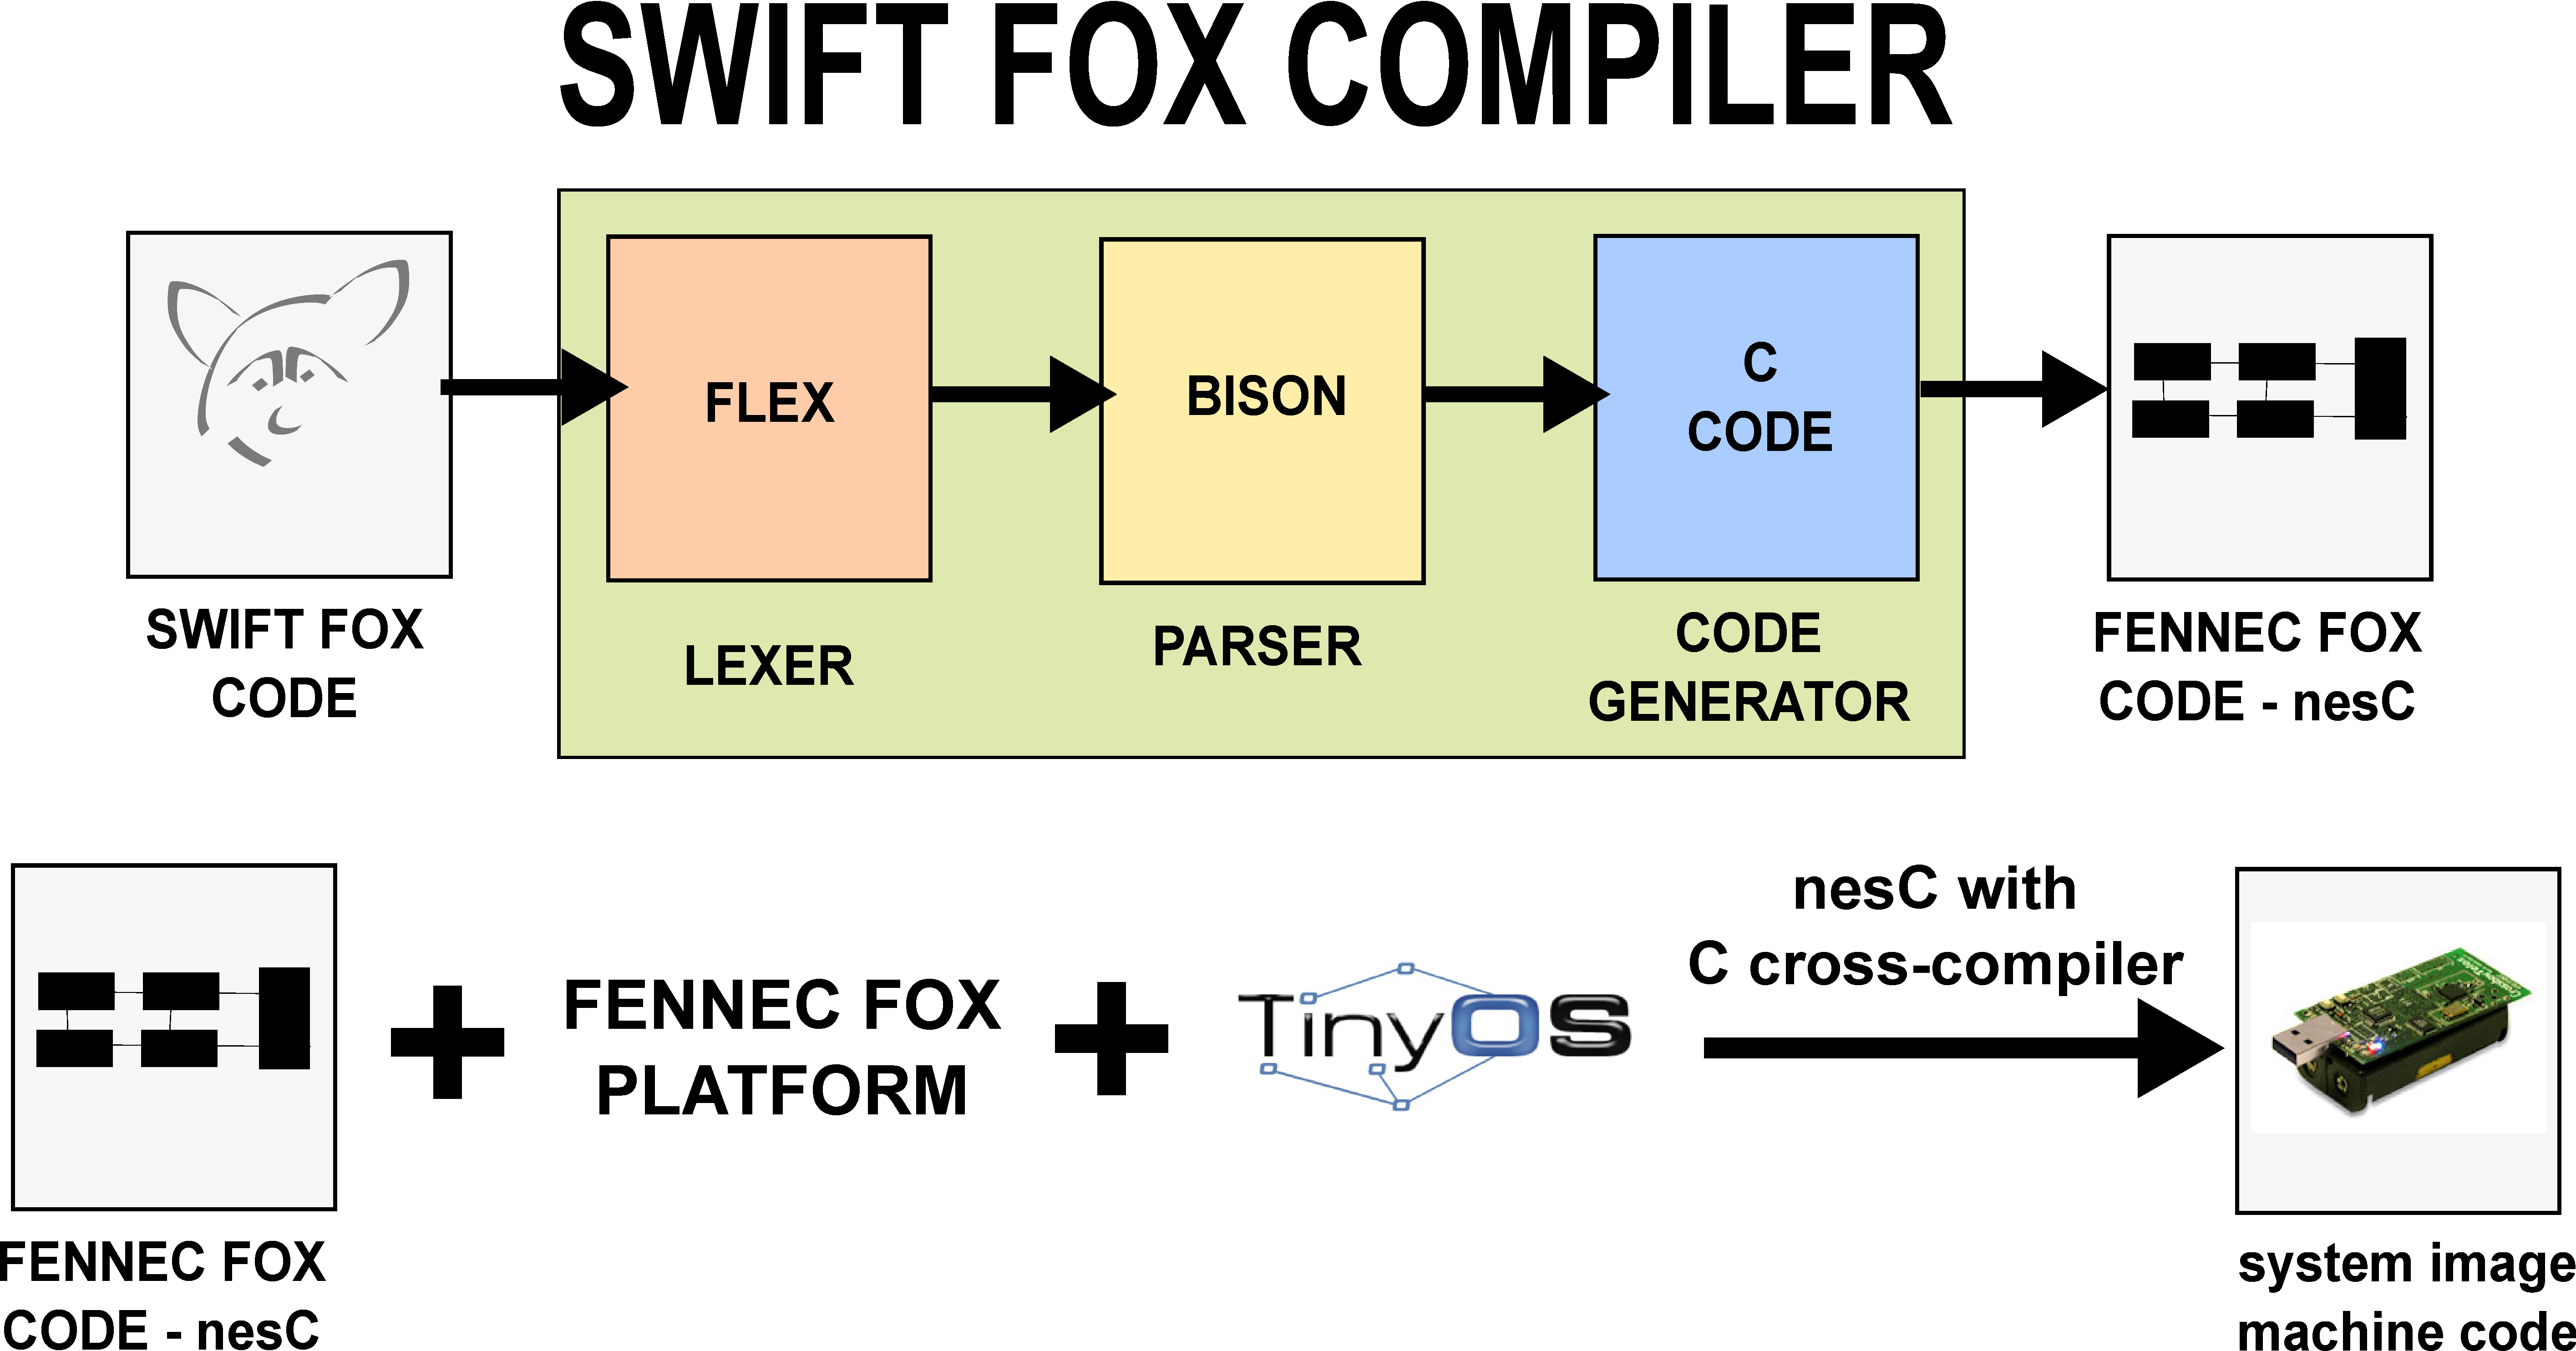
\includegraphics[scale=0.1]{fig/arch.pdf}
		\end{center}
		\caption{Swift Fox block diagram}
	\end{figure} 
\end{frame}

\subsection[Development]{Development tools}

\begin{frame}{Swift Fox}{Development tools}
	\begin{block}{development}
		\begin{itemize}
		\item Lex (flex), YACC (bison) 
		\item nesC, TinyOS
		\item make
		\end{itemize}
	\end{block}
	\begin{block}{management \& documentation}
		\begin{itemize}
		\item Trac (web-management and bug-tracking)
		\item Subversion (revision control)
		\item \LaTeX
		\end{itemize}
	\end{block}
\end{frame}

\subsection[Testing]{Testing tools}

\begin{frame}{Swift Fox}{Testing procedure}
	\begin{itemize}
	\item assume correctness of the front-end generators and execution
	environment (\textit{e.g.,} Lex, YACC, nesC, TinyOS, Fennec Fox)
	\item combination of \textit{unit} and \textit{regression} testing
	\item separate regression testing suites for the lexer, parser, and
	code generator
	\end{itemize}
\end{frame}


\section[Conclusion]{Conclusion (Xuan Linh Vu)}

\subsection[Lessons]{Lessons learned}

\begin{frame}{Swift Fox}{What we learned}
	\begin{itemize}
	\item testing is important
	\item keep it simple, add features steadily
	\item documentation helps!
	\item {\color{blue} project management is hard}
	\end{itemize}
\end{frame}

\subsection[Why Swift Fox]{Why Swift Fox}

\begin{frame}{Why Swift Fox?}
	\begin{itemize}
	\item first language (of that kind) out there
	\item simpler than coding in \textit{nesC}
	\item {\color{blue} solve the ``problem'' and avoid plumbing}
	\end{itemize}
	\begin{block}{Try it! (\textit{coming soon...})}
		\centering
		\url{http://nslvm2.cs.columbia.edu}
	\end{block}
\end{frame}


\end{document}
